\normaltrue \difficilefalse \tdifficilefalse
\correctiontrue

%\UPSTIidClasse{11} % 11 sup, 12 spé
%\renewcommand{\UPSTIidClasse}{12}

\exer{Poulie Redex $\star$ \label{C2:06:31}}
\marginnote{D'après ressources de Stéphane Genouël.}
\setcounter{question}{0}\marginnote{\UPSTIcompetence[2]{A3-05}
\UPSTIcompetence[2]{C2-06}}
\index{Compétence C2-06}
\index{Poulie Redex}
\ifcorrection
\else
\marginnote{\textbf{Pas de corrigé pour cet exercice.}}
\fi

\ifprof
\else
Soit le train d'engrenages suivant. 
\begin{center}
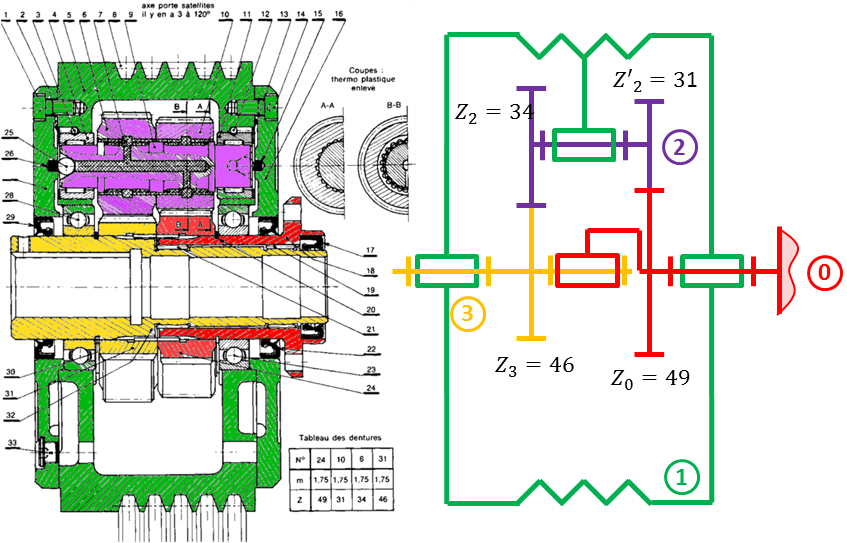
\includegraphics[width=\linewidth]{31_01}
\end{center}
\fi


\question{Tracer le graphe des liaisons.}
\ifprof
\else
\fi

\question{Déterminer littéralement, en fonction des nombres de dents, la loi E/S du système (c'est-à-dire le rapport de transmission).}
\ifprof ~\\
On cherche $\dfrac{\omega_{30}}{\omega_{10}}$. En bloquant le porte satellite 1, on a  
$\dfrac{\omega_{31}}{\omega_{01}}=\dfrac{Z_0 Z_2 }{Z_2' Z_3}$. En décomposant les vitesses, on a :
$\dfrac{\omega_{30}-\omega_{10}}{\omega_{10}}=-\dfrac{Z_0 Z_2 }{Z_2' Z_3}$
$\Leftrightarrow \omega_{30}-\omega_{10}=-\dfrac{Z_0 Z_2 }{Z_2' Z_3}\omega_{10}$
$\Leftrightarrow \omega_{30}=\left(1-\dfrac{Z_0 Z_2 }{Z_2' Z_3}\right)\omega_{10}$
$\Leftrightarrow \dfrac{\omega_{30}}{\omega_{10}}=1-\dfrac{Z_0 Z_2 }{Z_2' Z_3}$.

AN : $ \dfrac{\omega_{30}}{\omega_{10}}=1-\dfrac{49 \times 34}{31 \times 46}=-0,17$.à
\else
\fi


\ifprof
\else
\begin{flushright}
\footnotesize{Corrigé  voir \ref{C2:06:31}.}
\end{flushright}%
\fi